\documentclass[svgnames,smaller,table]{beamer}
\usepackage{multirow}
\usepackage{tikz}
\usefonttheme[onlymath]{serif}

\usepackage{listings}
% Configura o listings
\lstset{
  %  basicstyle=\footnotesize,\small,...\tiny
  basicstyle=\ttfamily\scriptsize,
  commentstyle=\color{mygreen},
  numbers=left,
  stepnumber=1,
  showstringspaces=false,
  tabsize=2,
  breaklines=true,
  breakatwhitespace=false
 columns=fixed,
 fontadjust=true,
 basewidth=0.5em
}


\usetheme{lthn}
\setbeamercolor*{normal text}{fg=black}
% -----------------------------------------------------------------------------------------------------------------

\title[Slide]{The Use of Serpent at the LTHN/CDTN}
\author{Vitor Vasconcelos A. Silva}
\date{\today}
\institute{%
  LTHN - Thermal-hydraulics and Neutronics Laboratory
  \par
  Reactors Technology Service - CDTN/CNEN}

\begin{document}

%-------------------------------------------------
\begin{frame}
\titlepage
\end{frame}

%-------------------------------------------------
\begin{frame}
  \frametitle{Summary}
  \tableofcontents%[pausesections]
\end{frame}


\section{CDTN}
%-------------------------------------------------
\begin{frame}
  \frametitle{CDTN}
  \framesubtitle{Nuclear Technology Development Center}
  \begin{center}
    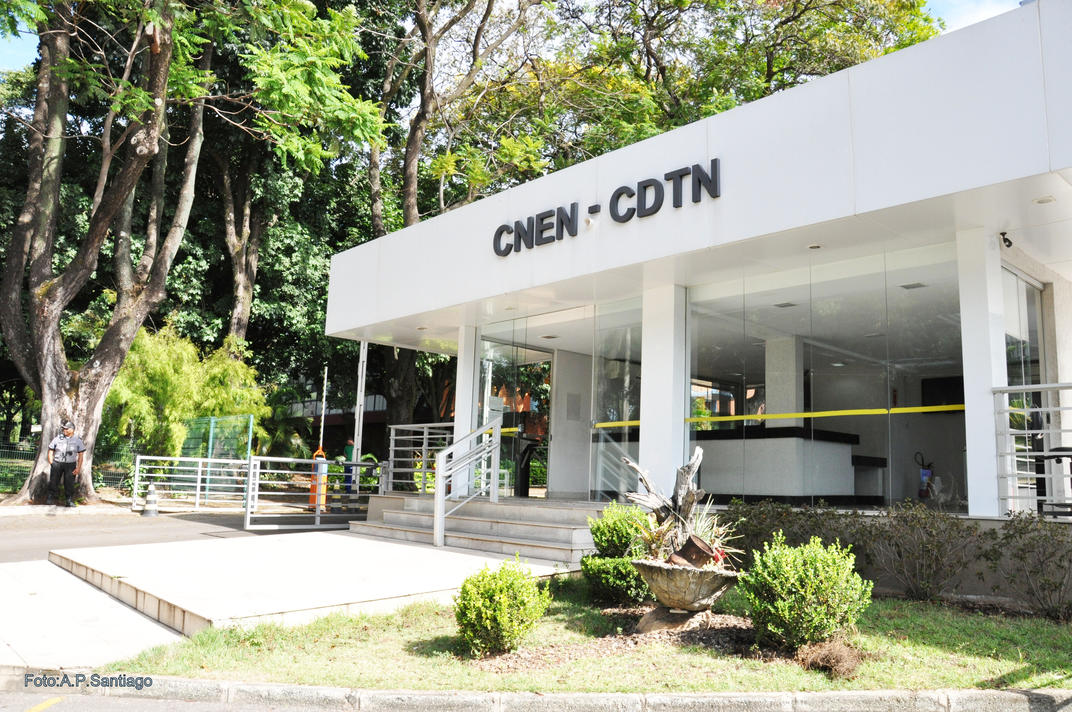
\includegraphics[scale=1.1]{figuras/portaria1_CDTN.jpg}
    \end{center}
\end{frame}

%-------------------------------------------------
\begin{frame}
  \frametitle{CDTN}
  \framesubtitle{Nuclear Technology Development Center}
    \begin{center}
      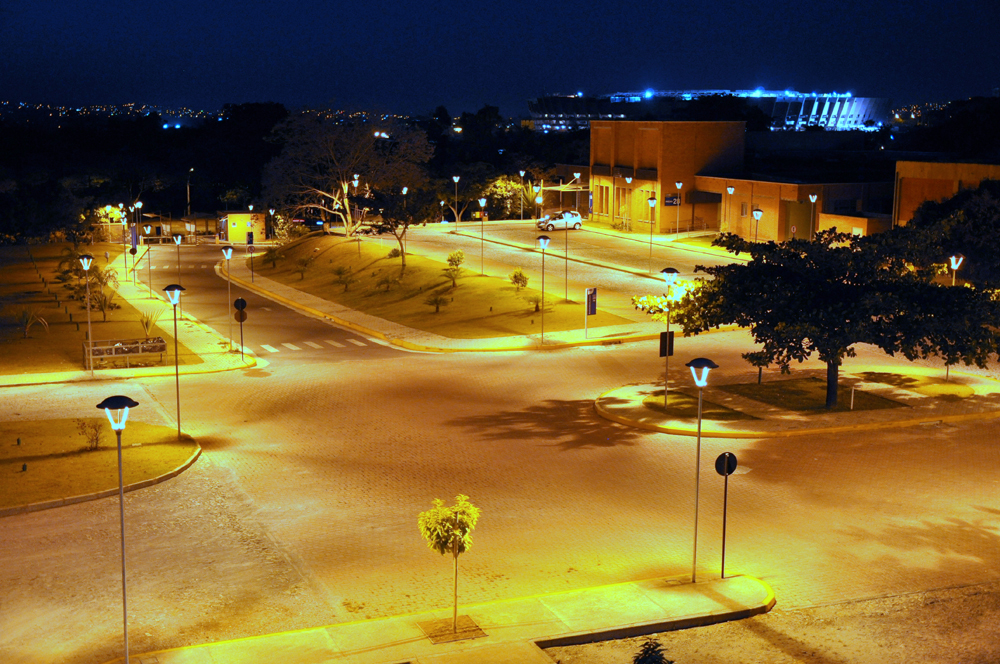
\includegraphics[scale=1.2]{figuras/predio_28_noite.jpg}
    \end{center}
\end{frame}

%-------------------------------------------------
\begin{frame}
  \frametitle{CDTN}
  \framesubtitle{Nuclear Technology Development Center}
  \begin{itemize}
  \item Founded in 1952 as IPR (Radioactive Research Institute), part of
    Minas Gerais Federal University.
  \item In 1960, TRIGA Mark 1 reactor inaugurated - first criticality.
  \item Many areas...
    \item Neutronics + thermal....
  \end{itemize}
\end{frame}


\section{Thermal-Hydraulics and Neutronics Lab - LTHN}
%-------------------------------------------------
\begin{frame}
  \frametitle{Thermal-Hydraulics and Neutronics Lab - LTHN}
  \framesubtitle{Experimental facilities}
  \begin{center}
    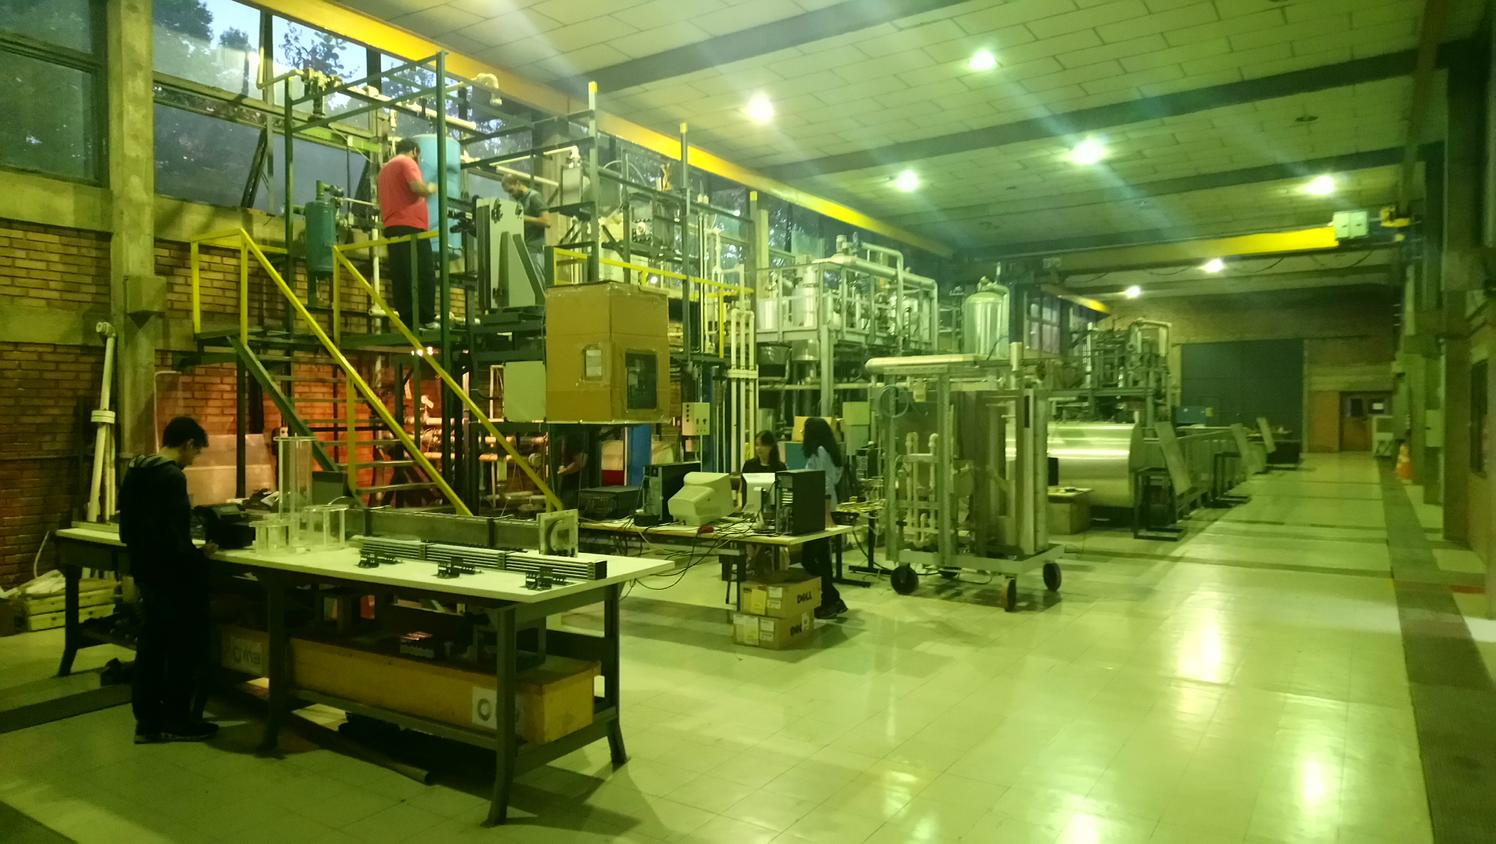
\includegraphics[scale=0.2]{figuras/labth.jpg}
  \end{center}
\end{frame}

\begin{frame}
  \frametitle{Thermal-Hydraulics and Neutronics Lab - LTHN}
  \framesubtitle{Computer Laboratory}
  \begin{center}
    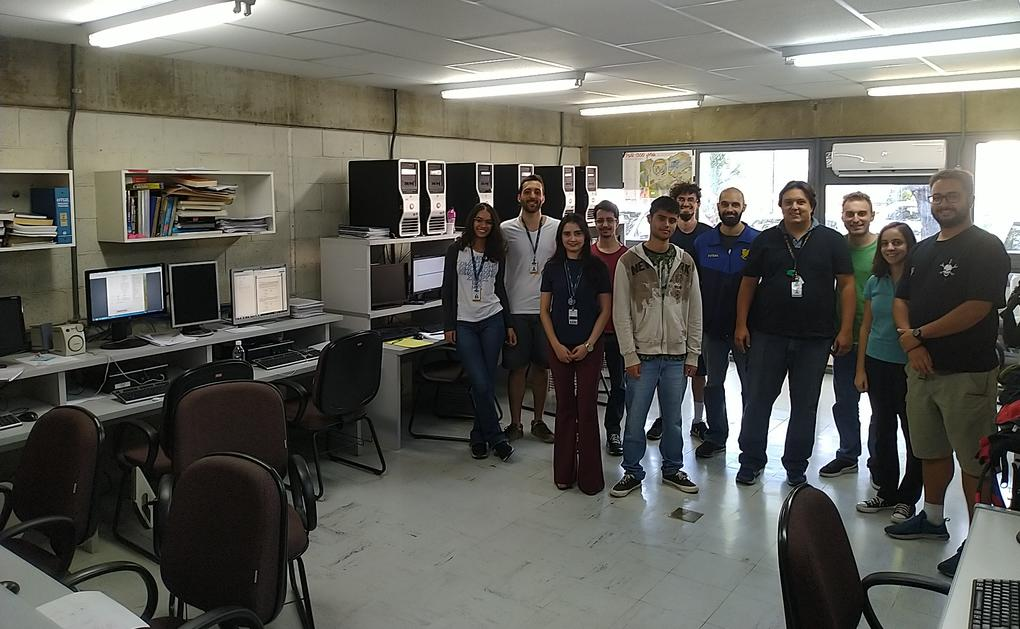
\includegraphics[scale=0.3]{figuras/lthn-computers-cropped.jpg}
  \end{center}
\end{frame}

%-------------------------------------------------
\begin{frame}
  \frametitle{Thermal-Hydraulics and Neutronics Lab - LTHN}
  \framesubtitle{Main activities}
  \begin{center}
    \begin{itemize}
    \item Experimental thermal-hydraulics: spacer grids, counter current fluid flow, PIV;
    \item IPR-R1 TRIGA modelling, uncertainty propagation in MC simulations;
    \item Fusion-fission simulations, advanced fuel burn-up (\textbf{SERPENT});
    \item Software development $\star$;
    \end{itemize}
  \end{center}
\end{frame}

\section{Monte Carlo simulation work}
%-------------------------------------------------
\begin{frame}
  \frametitle{Monte Carlo simulation work}
  \framesubtitle{Serpent2 use}
  \textbf{Monte Carlo}
    \begin{itemize}
    \item RMB
    \item Novos combustiveis...
    \item Fusao...
    \end{itemize}
    \vspace{10px}
  \textbf{Algo aqui?}
    \begin{itemize}
    \item bla
    \end{itemize}
\end{frame}

\subsection{Tiago - acoplamento}
%-------------------------------------------------
\begin{frame}
  \frametitle{OpenFOAM + Serpent2 coupling}
  \framesubtitle{Objective}
  \begin{center}
    Fidelity on the simulation of nuclear systems\\
    \vspace{10px}
    \begin{itemize}
    \item RMB: Brazilian Multipurpose Reactor $\rightarrow$ under design.
    \item Why CFD + Monte Carlo $\rightarrow$ High accuracy level.
    \item Initialy simplifed model $\rightarrow$ fuel pin.
    \end{itemize}
    But why modelling a fuel pin for a plate fuel reactor?
    \begin{itemize}
    \item Previous work (citar paper annals): tested mesh for a \textbf{TRIGA} pin
    \item Straighforward to extend the methodology to MC approach
    \item Low computational cost
    \end{itemize}
  \end{center}
\end{frame}

\begin{frame}
  \frametitle{OpenFOAM + Serpent2 coupling}
  \framesubtitle{Results}
  \begin{center}
%    \includegraphics[scale=0.2]{figuras/esquema.png}
    
  \end{center}
\end{frame}

\begin{frame}[fragile] % Coloca isso no frame que tem verbatim
  \frametitle{OpenFOAM + Serpent2 coupling}
  \framesubtitle{Current problems}
  \begin{center}
  Zirconium hydride: pin initially modelled as TRIGA fuel.\\
\begin{verbatim}
  Fatal error in function OTFSabScattering:

  Energy grids differ in OTF S(a,b) interpolation

  Simulation aborted.
\end{verbatim}

On file \texttt{otfsabscattering.c} we got:

%\begin{verbatim}
%              /* NOTE: tää on kohtuullisen harvinainen sirontalaki, johon */
%              /* törmää esim. h/zr ja zr/h -kirjastoissa. Ei ole kunnolla */
%              /* testattu. */
%\end{verbatim}
  
  \end{center}
\end{frame}


\begin{frame}
  \frametitle{OpenFOAM + Serpent2 coupling}
  \framesubtitle{Problems}
  \begin{center}
    

  \end{center}
\end{frame}


% END SUBSECTION----------------------------------

\subsection{NPS}
%-------------------------------------------------
\begin{frame}
  \frametitle{NPS}
  \framesubtitle{}
%We are using SERPENT in external source mode to simulate a hybrid system fusion-fission. The geometry simulated is based on concentrically spheres, where there are nine zones filled with the RFS with thorium and ten zones with coolant Li$_{17}$Pb$_{83}$. The source was produced by the D-T fusion reaction generating neutrons of $14.1$ MeV and placed in the central sphere with a radius of 250 cm, as shown in Figure \ref{fusion}.

\frametitle{}
  \framesubtitle{View}
  \begin{center}
    
\includegraphics[scale=0.4]{figuras/fusion.png}
%    \caption{Fusion system geometry.}
    \label{fusion}
  \end{center}
\end{frame}


%-------------------------------------------------
\begin{frame}
  \frametitle{NPS}
  \framesubtitle{Current Problems}
  
%We are having problems to understand how NPS value influences the results of k$_{eff}$(analog) in those simulations. It was noticed that the values of k$_{eff}$(analog) increases considerably when the value of NPS is also increased. Even for high values of NPS (larger than 500000), the values of  k$_{eff}$(analog) obtained for various NPS are considerably different. Table \ref{NPS} shows the k$_{eff}$(analog) values obtained for several NPS values.

\begin{table}[htb!]
\caption{k$_{eff}$ Results for different NPS}
\label{NPS}
\centering
\vspace{0.5cm}
\begin{tabular}{c|c|c}\hline
NPS & k$_{eff}$(analog) & 95\% confidence interval\\ \hline

$10000$ & $0.59490$ & $0.53182-0.65798$\\ \hline
$20000$ & $0.69282$ & $0.64750-0.73802$\\ \hline
$30000$ & $0.74796$ & $0.71240-0.78352$\\ \hline
$40000$ & $0.77101$ & $0.74249-0.79953$\\ \hline
$50000$ & $0.76816$ & $0.73942-0.79690$\\ \hline
$60000$ & $0.79388$ & $0.76734-0.82042$\\ \hline
$100000$ & $0.82596$ & $0.80478-0.84714$\\ \hline
${\bf 500000}$ & $0.88611$ & $0.87775-0.89447$\\ \hline
${\bf 1000000}$ & $0.89095$ & $0.88547-0.89643$\\ \hline
${\bf 10000000}$ & $0.90109$ & $0.89905-0.90313$\\ \hline
${\bf 20000000}$ & $0.90142$ & $0.90012-0.90272$\\ \hline
\end{tabular}
\end{table}

Similar behavior is verified when we use SERPENT to simulate ADS. Is there a limit inferior to NPS?
\end{frame}


%-------------------------------------------------
%\begin{frame}
%  \frametitle{Neutron Extractor}
%  \framesubtitle{Technical aspects related to neutrongraphy}
%    \begin{itemize}
%    \item Collimation ratio: \scalebox{1}{$\left(\frac{L}{D}\right)=\frac{460cm}{10cm}=46$}
%    \item Neutron to gamma ratio: \scalebox{1.5}{$\frac{n}{\gamma}$} $ = 153 \times 10^4 (mR)^{-1}.cm^{-2}$ \textsuperscript{[}\footnote{A. L. Costa, 2003}\textsuperscript{]} 
%    \item Only one report on thermal/epithermal neutrons (Cd) ratio: at 3.6 meters over reactor's graphite reflector it is $27$. (Information only) 
%    \end{itemize}
%    \vspace{10px}
%\end{frame}

\section{Conclusions}
%-------------------------------------------------
\begin{frame}
  \frametitle{Conclusions}
  \framesubtitle{And some future intentions}
  Roughly, half of the activities of neutronic modelling and simulation at the LTHN are done using Serpent2.
\end{frame}



%-------------------------------------------------
% FIM
%-------------------------------------------------
\begin{frame}
 \vfill
  \begin{beamercolorbox}[center]{title}
     \Huge{Thank you!}
  \end{beamercolorbox}
  \vfill
\end{frame}


\end{document}

